\definecolor{forestgreen(web)}{rgb}{0.13, 0.55, 0.13}
\definecolor{ao}{rgb}{0.0, 0.0, 1.0}
\definecolor{burgundy}{rgb}{0.5, 0.0, 0.13}
\definecolor{byzantium}{rgb}{0.44, 0.16, 0.39}
\chapter{Design of the RV32I Machine}
	\minitoc
	\vspace{5mm}
	In this chapter, as mentioned before, we will present one by one the CPU's pipeline stages and also the final design. Every part and every module that was created (via $VHDL$) was thoroughly tested before moving to the next one. The whole design consists of five pipeline stages which are the Instruction Fetch, the Instruction Decode, Execute Stage, Memory Stage and Write Back Stage. 
	\clearpage
	\section{Instruction Fetch - IF}
	 \label{Instruction Fetch}
	 The Instruction Fetch ($IF$) module consists of a simple memory block (M4K - block)\footnote{The use of M4K was mandatory in our case since we wanted the design to be synthesizable. Having that in mind, the only embedded memory available on our FPGA board was the M4K RAM memory type } that is used to simulate the Instruction Cache (I\$) in our system. 
	 We chose for the I\$ to have $1024$ slots which are $32$-bit wide (since we are implementing a 32-bit architecture). So the total capacitance of the memory is $4096$ B. 
	 
	 \begin{figure}[h!]
	 	\begin{center}
	 		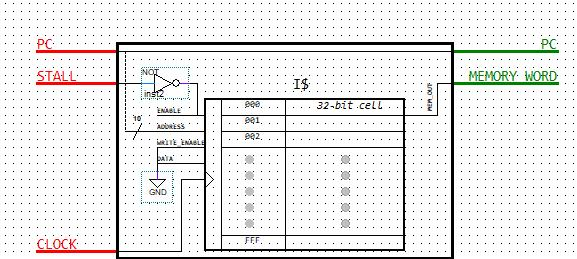
\includegraphics[width=1\textwidth]{IF}
	 		\caption{Instruction Fetch schematic}
	 		\label{Image3.1}
	 	\end{center}
	 \end{figure}
 
	 $IF$ is responsible for fetching the proper instruction ($MEMORY\_WORD$) from I\$. This is done by isolating some bits of the program counter ($PC$) and using them as address for the I\$. Since the memory has $1024$ slots we need $\log_2(1024)=\underline{10}$ bits to iterate through all of them and so, we use the $PC(11..2)$ bits for this work. \\
	 Module's I/O:	  
	
	 {\small
 	 \renewcommand{\labelenumii}{\Roman{enumii}}
	 \begin{itemize}
	 	\item Inputs:
	 	\begin{enumerate}
	 		
	 		\item \textcolor{red}{$CLOCK$} : System clock.
	 		\item \textcolor{red}{$STALL$} : Pipeline control signal (1-bit).
	 		\item \textcolor{red}{$PC$}    : Program counter (32-bit).
	 	\end{enumerate}
 		\item Outputs:
 		\begin{enumerate}
 		
 			\item \textcolor{forestgreen(web)}{$MEMORY\_WORD$} : Word fetched from I\$ (32-bit).
 			\item \textcolor{forestgreen(web)}{$PC$}	 	   : Program counter (32-bit).
 		\end{enumerate}
	 \end{itemize}}
 	\vspace{5mm}
 	 	
 	Last but not least the M4K Memory used was automatically generated by Quartus's II Mega-Wizard Plug-In Manager.
 	
 	\newpage
 	
 	\section{Instruction Decode - ID}
 	\label{Instruction Decode}
 	This is one of the most important and resourceful modules of this design. The Instruction Decode ($ID$) module is responsible for one thing among others; to "recognize" the command that was fetched on the previous cycle and activate all the signals that are needed for the command to be successfully processed.
 	
 		 \begin{figure}[h!]
 		\begin{center}
 			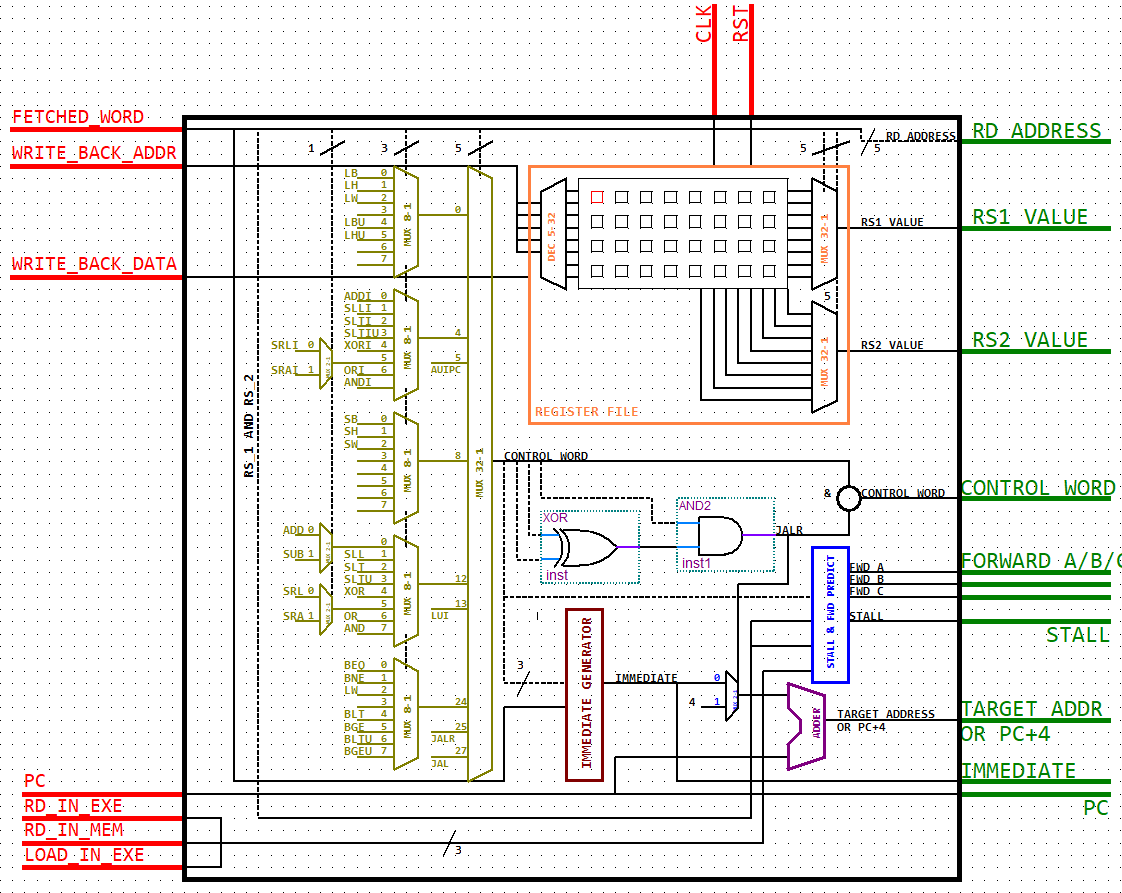
\includegraphics[width=1.0\textwidth]{DECODE}
 			\caption{Instruction Decode schematic}
 			\label{Image3.2}
 		\end{center}
 	\end{figure}
 	
 	\vspace{2mm}
 	
 	Designing the $ID$ module was a trial-and-error process due to the nature of the task that is asserted to it. While being the second part of the pipeline, its development suggests a deep knowledge of what will be done in one, two, and three clock cycles later for every(!) command that is currently being decoded. In this stage we also detect true dependencies ($RAWs$ %sto telos episis
 	) and handle them accordingly to maximize the performance when it is needed. Also, ID is being equipped with a simple \textcolor{byzantium}{Adder} so that it can calculate either the return address of a $JUMP$ or the target address ($PC+IMMEDIATE$) according to the Uncoditional Jump command that is currently being decoded. \\\\
 	Once again, we will follow the color-code of Figure \ref{Image3.2} so one can navigate through the design and the description.
 	
 	\clearpage
 	
 	\subsection{\textcolor{olive}{Multiplexer Network}}
 	\label{subsubsection3.2.1}
 	
 	Being tasked with the work of decoding the previously fetched instruction (\textbf{word}), we have to figure out a way to detect which one of the possible instructions it is. After the successful decode of the word, we have to provide all(!) the mandatory \textbf{control signals} for the next pipeline stages to make sure that all the necessary actions for the process of the now decoded instruction will be done.\\\\ At Section \ref{sect2.3.3} we listed all the instructions that belong to our $RV32I$ implementation. Also, Figure \ref{Image2.2} shows that all the instruction types have their 7 LSBs\footnote{Least Significant Bits} dedicated for the $opcode$ field. Also, in combination with Figure \ref{image2.1} we conclude that there is no point to process the two LSBs of any word that has to be decoded.\\\\
 	The first step for the process is to understand how the commands are being encoded by the Assembler; and to do so we used the official RISC-V Instruction Set Manual. The encoding of every command is displayed below at Table \ref{subsec3.2:table3.1}. Marked with bold style is all the information the Multiplexer Network uses to determine the identity of the command.
 	
 	Observing the encoding information displayed on Table \ref{subsec3.2:table3.1} we came to the following conclusions:
 	\begin{itemize}
 		\item According to their $opcode$ bits the commands are either stand-alone or belong in a group with other commands of similar type or functionality.
 		\item The groups are the following five:
 		\begin{itemize}
 			\item Loads
 			\item I-type arithmetics
 			\item Stores
 			\item R-type commands
 			\item Branches
 		\end{itemize}
 		\item Most of the commands that belong to a group, have a "unique" $funct3$ 3-bit code. 
 		\item Some of the grouped commands have the same $funct3$ code but have a different $funct7[5]$ bit.
 	\end{itemize}	
 	\vspace{2mm}
 	
 		 In conclusion the Multiplexer Network is responsible of selecting the correct control signal to pass to the following pipeline stages. Each multiplexer's input is a static control signal, which dictates what operations must be done in every stage for the successful process of the command. 
		
	\clearpage
	
 	\vspace{2mm}
 	\begin{threeparttable}[h!]
 		
	 	\begin{tabular}{|c|c|c|c|c|c|r|} \hline
	 	\multicolumn{4}{|c|}{imm[31:12]}	   &	rd	        & \textbf{01101}11                   & "LUI"                     \\\Xhline{5\arrayrulewidth}
	 	\multicolumn{4}{|c|}{imm[31:12]}	   &	rd	        &\textbf{00101}11                    & "AUIPC"                   \\\Xhline{5\arrayrulewidth}
	 	
	 	\multicolumn{4}{|c|}{imm[20\&10:1\&11\&19:12]}	& rd	&\textbf{11011}11 				     & "JAL" 				    \\\Xhline{5\arrayrulewidth}
	 	
	 	\multicolumn{2}{|c|}{imm[11:0] }       &	rs1	& 000	& rd  & \textbf{11001}11        	 & "JALR" 					\\\Xhline{5\arrayrulewidth}
	 	
	 	imm[12\&10:5] 						   & 	rs2	& rs1	& \setrow{\bfseries}000 & 	imm[4:1\&11]  	& \textbf{11000}11	& "BEQ" 		\\\hline
	 	imm[12\&10:5] 						   & 	rs2	& rs1	& \setrow{\bfseries}001 & 	imm[4:1\&11] 	& \textbf{11000}11	& "BNE" 		\\\hline
	 	imm[12\&10:5] 						   & 	rs2	& rs1	& \setrow{\bfseries}100 & 	imm[4:1\&11] 	& \textbf{11000}11	& "BLT" 		\\\hline
	 	imm[12\&10:5] 						   & 	rs2	& rs1	&\setrow{\bfseries} 101 & 	imm[4:1\&11] 	& \textbf{11000}11	& "BGE" 		\\\hline
	 	imm[12\&10:5] 						   & 	rs2	& rs1	& \setrow{\bfseries}110 & 	imm[4:1\&11] 	& \textbf{11000}11	& "BLTU" 		\\\hline
	 	imm[12\&10:5] 						   & 	rs2	& rs1	&\setrow{\bfseries} 111 & 	imm[4:1\&11] 	& \textbf{11000}11	& "BGEU" 		\\\Xhline{5\arrayrulewidth}
	 	
	 	\multicolumn{2}{|c|}{imm[11:0]}        &   rs1 & \setrow{\bfseries}000   & rd & \textbf{00000}11 & "LB"  \\\hline
	 	\multicolumn{2}{|c|}{imm[11:0]}		   &   rs1 & \setrow{\bfseries}001   & rd & \textbf{00000}11 & "LW"  \\\hline
	 	\multicolumn{2}{|c|}{imm[11:0]}        &   rs1 & \setrow{\bfseries}010   & rd & \textbf{00000}11 & "LW"  \\\hline
	 	\multicolumn{2}{|c|}{imm[11:0]}  	   & 	rs1 & \setrow{\bfseries}100  & rd & \textbf{00000}11 & "LBU" \\\hline
	 	\multicolumn{2}{|c|}{imm[11:0]} 	   &   rs1 & \setrow{\bfseries}101   & rd & \textbf{00000}11 & "LHU" \\\Xhline{5\arrayrulewidth}
	 	
	 	imm[11:5] & rs2 & rs1 & \setrow{\bfseries}000 & imm[4:0] & \textbf{01000}11 & "SB" \\\hline
	 	imm[11:5] & rs2 & rs1 & \setrow{\bfseries}001 & imm[4:0] & \textbf{01000}11 & "SH" \\\hline
	 	imm[11:5] & rs2 & rs1 & \setrow{\bfseries}010 & imm[4:0] & \textbf{01000}11 & "SW" \\\Xhline{5\arrayrulewidth}
	 	
		\multicolumn{2}{|c|}{imm[11:0]} & rs1 & \setrow{\bfseries}000 & rd &\textbf{00100}11 & "ADDI"  \\\hline
		\multicolumn{2}{|c|}{imm[11:0]} & rs1 & \setrow{\bfseries}010 & rd &\textbf{00100}11 & "SLTI"  \\\hline
		\multicolumn{2}{|c|}{imm[11:0]} & rs1 & \setrow{\bfseries}011 & rd &\textbf{00100}11 & "SLTIU" \\\hline
		\multicolumn{2}{|c|}{imm[11:0]} & rs1 & \setrow{\bfseries}100 & rd &\textbf{00100}11 & "XORI"  \\\hline
		\multicolumn{2}{|c|}{imm[11:0]} & rs1 & \setrow{\bfseries}110 & rd &\textbf{00100}11 & "ORI"   \\\hline
		\multicolumn{2}{|c|}{imm[11:0]} & rs1 & \setrow{\bfseries}111 & rd &\textbf{00100}11 & "ANDI"  \\\hline
		0000000 & shamt & rs1 & \setrow{\bfseries}001 & rd &\textbf{00100}11 & "SLLI" \\\hline
		0000000 & shamt & rs1 & \setrow{\bfseries}101 & rd &\textbf{00100}11 & "SRLI" \\\hline
		0\textbf{1}00000 & shamt & rs1 & \setrow{\bfseries}101 & rd & \textbf{00100}11 & "SRAI" \\\Xhline{5\arrayrulewidth}
		
		0000000 & rs2   & rs1 & \setrow{\bfseries}000 & rd & \textbf{01100}11 & "ADD"  \\\hline
		0\textbf{1}00000 & rs2   & rs1 & \setrow{\bfseries}000 & rd & \textbf{01100}11 & "SUB"  \\\hline
		0000000 & rs2   & rs1 & \setrow{\bfseries}001 & rd & \textbf{01100}11 & "SLL"  \\\hline
		0000000 & rs2   & rs1 & \setrow{\bfseries}010 & rd & \textbf{01100}11 & "SLT"  \\\hline
		0000000 & rs2   & rs1 & \setrow{\bfseries}011 & rd & \textbf{01100}11 & "SLTU" \\\hline
		0000000 & rs2   & rs1 & \setrow{\bfseries}100 & rd & \textbf{01100}11 & "XOR"  \\\hline
		0000000 & rs2   & rs1 & \setrow{\bfseries}101 & rd & \textbf{01100}11 & "SRL"  \\\hline
		0\textbf{1}00000 & rs2   & rs1 & \setrow{\bfseries}101 & rd & \textbf{01100}11 & "SRA"  \\\hline
		0000000 & rs2   & rs1 & \setrow{\bfseries}110 & rd & \textbf{01100}11 & "OR"   \\\hline
		0000000 & rs2   & rs1 & \setrow{\bfseries}111 & rd & \textbf{01100}11 & "AND"  \\\hline
	 	\end{tabular}
 		
 		\begin{tablenotes}
 		\footnotesize
 		\item 
 		Notes:
 		\item 	
 		"\&" is the concatenation operator.
 		\end{tablenotes}
 		
 		\captionof{table}{RV32I Command Encoding}
 		\label{subsec3.2:table3.1}
 		\vspace{5mm}
 		
 	\end{threeparttable}
 
 	\clearpage
	 	 
	 Starting from right to left, there is a $32\rightarrow1$ multiplexer. This multiplexer is used to select the correct group of the command (if the command belongs to a group) or the stand-alone command itself(e.g. "AUIPC"). This is done by using the $opcode[6..2]$ bits of the word as selector. Since the $opcode[6..2]$ bits alter from command to command in a non-sequential manner, we use all five of them and end up with a $2^{5}=32\rightarrow1$ multiplexer.\\
	 
	 Following behind, there are five $8\rightarrow1$ multiplexers which use the three $funct3$ bits (if any) of the word to select a specific command inside a group. Note that since we have five different command groups, we use five multiplexers in this layer.\\
	 
	 Some of the commands, belong to the same group and also have the same $funct3$ code (e.g. "ADD" - "SUB"). To separate them we utilize the $funct7[5]$ bit of the word which changes in that case. So, using this bit as selector we attach to the network three $2\rightarrow1$ multiplexers and so, we cover all the possible scenarios of decoding.\\
	 
	
	\subsubsection{Multiplexer Input}
	\label{subsub:muxin}
	
	As mentioned above, the input of every multiplexer is a static, hard-typed control signal of $20$ bits of the following format. \\
	
	\begin{figure}[h!]
		\begin{center}
			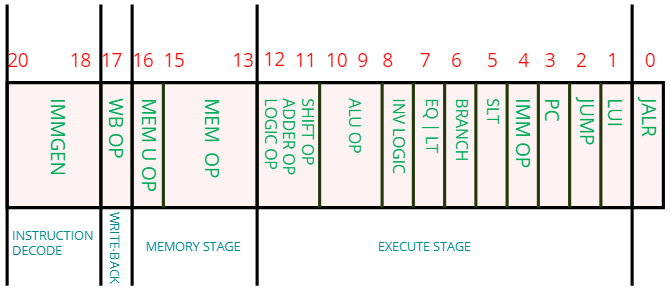
\includegraphics[width=0.7\textwidth]{ControlWord}
			\caption{Control Word Format}
			\label{Image3.3}
		\end{center}
	\end{figure}	

	\vspace{2mm}
	
	Depicted with blue color at Figure \ref{Image3.3} are four groups of bits. These are the bits that concern each pipeline stage. The bit $0$ is used also at ID stage along with bits $20..18$ but it is appended later as Figure \ref{Image3.2} shows and is not hard-type in every input of the multiplexers like the rest of the control signal bits. It is also used for pipeline control.
	
	\clearpage
	\small
	\begin{itemize}
		%\setlength\itemsep{-0.1em}
		\item \textbf{IMMGEN} : Immediate Genaration
		\begin{itemize}
			\setlength\itemsep{-0.1em}
			\item $000$ : I-type Immediate,
			\item $001$ : S-type Immediate.
			\item $010$ : B-type Immediate.
			\item $011$ : U-type Immediate.
			\item $100$ : J-type Immediate.
		\end{itemize}
		\item \textbf{WB OP} : Write Back operation. $0$ if the command doesn't require a Write Back action, $1$ if it does.
		\item \textbf{MEM U OP} : Memory Unsigned Operation. $0\rightarrow NO$, $1\rightarrow YES$.
		\item \textbf{MEM OP} : Memory Operation.
		\begin{itemize}
			\setlength\itemsep{-0.1em}
			\item $000$ : LB 
			\item $001$ : LH
			\item $010$ : LW
			\item $100$ : SB
			\item $101$ : SH
			\item $110$ : SW
			\item $111$ : MEM-Free operation.
		\end{itemize}
		\item \textbf{ALU OP}: ALU Operation 
		\begin{itemize}
			\setlength\itemsep{-0.1em}
			\item $00$ : Addition.
			\item $01$ : Subtraction.
			\item $10$ : Logic Operation.
			\item $11$ : Shift Operation.
		\end{itemize}
		\item \textbf{SHIFT/ADDER/LOGIC OP}: Since bits $[9..8]$ determine which ALU module will be used there is no problem using the same bits $[11..10]$ to represent different operations in different ALU modules. 
		\begin{itemize}
			\setlength\itemsep{-0.3em}
			\item Shift Module:
			\begin{itemize}
				\setlength\itemsep{-0.1em}
				\item $00$ : Shift Right Logical.
				\item $01$ : Shift Left Logical.
				\item $10$ : Shift Right Arithmetic.
			\end{itemize}
			\item Adder Module:
			\begin{itemize}
				\setlength\itemsep{-0.1em}				
				\item $0X$ : Signed Addition or Subtraction.
				\item $1X$ : Unsigned Addition or Subtraction.

			\end{itemize}
			\item Logic Module:
			\begin{itemize}
				\setlength\itemsep{-0.1em}
				\item $00$ : And.
				\item $01$ : Or.
				\item $10$ : Xor.			
			\end{itemize}
		\end{itemize}
		
		\item \textbf{INV}\textbf{ \& EQ/LT}: Used for resolving a branch case. 
		\item \textbf{BRANCH}: $0\rightarrow$ the command is not a Branch, $1\rightarrow$ the command is a Branch.
		\item \textbf{SLT}: $0\rightarrow$ the command is not SLT, $1\rightarrow$ the command is SLT.
		\item \textbf{PC}: $0\rightarrow$ PC is not required for calculations. $1\rightarrow$ PC is required for calculations.
		\item \textbf{JUMP}: $0\rightarrow$ the command is not a JUMP. $1\rightarrow$ command is a JUMP.
		\item \textbf{LUI}: $0\rightarrow$ the command is not a LUI. $1\rightarrow$ the command is a LUI.
		\item \textbf{JALR}: $0\rightarrow$ the command is not a JALR. $1\rightarrow$ the command is a JALR.
	\end{itemize}
	
	\clearpage
		
	\begin{center}
		\begin{threeparttable}[!ht]
			\begin{tabular}{|c|c|} \hline
				
				\setrow{\bfseries}Command &\setrow{\bfseries} Control-Word \\\hline
				LB   &000-1-0-000-0X-00-X-X-0-0-1-0-0-0-0 \\\hline
				LH   &000-1-0-001-0X-00-X-X-0-0-1-0-0-0-0\\\hline
				LW   &000-1-0-010-0X-00-X-X-0-0-1-0-0-0-0\\\hline
				LBU  &000-1-1-000-0X-00-X-X-0-0-1-0-0-0-0\\\hline
				LHU  &000-1-1-001-00-00-X-X-0-0-1-0-0-0-0\\\Xhline{5\arrayrulewidth}
				
				ADDI &000-1-X-111-0X-00-X-X-0-0-1-0-0-0-0\\\hline
				SLLI &000-1-X-111-01-11-X-X-0-0-1-0-0-0-0\\\hline
				SLTI &000-1-X-111-0X-01-X-X-0-1-1-0-0-0-0\\\hline 
				SLTIU&000-1-X-111-1X-01-X-X-0-1-1-0-0-0-0\\\hline 
				XORI &000-1-X-111-10-10-X-X-0-0-1-0-0-0-0\\\hline 
				SRLI &000-1-X-111-00-11-X-X-0-0-1-0-0-0-0\\\hline
				SRAI &000-1-X-111-10-11-X-X-0-0-1-0-0-0-0\\\hline
				ORI  &000-1-X-111-01-10-X-X-0-0-1-0-0-0-0\\\hline
				ANDI &000-1-X-111-00-10-X-X-0-0-1-0-0-0-0\\\Xhline{5\arrayrulewidth}
				
				SB &001-0-0-100-0X-00-X-X-0-0-1-0-0-0-0\\\hline
				SH &001-0-0-101-0X-00-X-X-0-0-1-0-0-0-0\\\hline
				SW &001-0-0-110-0X-00-X-X-0-0-1-0-0-0-0\\\Xhline{5\arrayrulewidth}
				
				ADD &XXX-1-X-111-0X-00-0-0-0-0-0-0-0-0-0\\\hline
				SUB &XXX-1-X-111-0X-01-0-0-0-0-0-0-0-0-0\\\hline
				SLL &XXX-1-X-111-01-11-0-0-0-0-0-0-0-0-0\\\hline
				SLT &XXX-1-X-111-0X-01-0-0-0-1-0-0-0-0-0\\\hline
				SLTU&XXX-1-X-111-1X-01-0-0-0-1-0-0-0-0-0\\\hline
				XOR &XXX-1-X-111-10-10-0-0-0-0-0-0-0-0-0\\\hline
				SRL &XXX-1-X-111-00-11-0-0-0-0-0-0-0-0-0\\\hline
				SRA &XXX-1-X-111-10-11-0-0-0-0-0-0-0-0-0\\\hline
				OR  &XXX-1-X-111-01-10-0-0-0-0-0-0-0-0-0\\\hline
				AND &XXX-1-X-111-00-10-0-0-0-0-0-0-0-0-0\\\Xhline{5\arrayrulewidth}
				
				BEQ &010-0-X-111-0X-01-0-1-1-0-0-0-0-0-0\\\hline
				BNE &010-0-X-111-0X-01-1-1-1-0-0-0-0-0-0\\\hline
				BLT &010-0-X-111-0X-01-0-0-1-0-0-0-0-0-0\\\hline
				BGE &010-0-X-111-0X-01-1-0-1-0-0-0-0-0-0\\\hline
				BLTU&010-0-X-111-1X-01-0-0-1-0-0-0-0-0-0\\\hline
				BGEU&010-0-X-111-1X-01-1-0-1-0-0-0-0-0-0\\\Xhline{5\arrayrulewidth}
				
				AUIPC&011-1-X-111-0X-00-X-X-0-0-1-1-0-0-0\\\hline
				LUI  &011-1-X-111-XX-00-X-X-0-0-1-1-0-1-0\\\hline
				JALR &000-1-X-111-01-00-X-X-0-0-1-0-1-0-1\\\hline
				JAL  &100-1-X-111-0X-00-X-X-0-0-1-1-1-0-0\\\Xhline{5\arrayrulewidth}
										
			\end{tabular}
				\begin{tablenotes}
				\footnotesize
				\item 
				Notes:
				\item 	
				"X" stands for "Don't Care". It could be either 1 or 0.
				\end{tablenotes}
				
			 	\captionof{table}{Commands and their Control-Words}
				\label{subsec3.2:table3.2}
				\vspace{3mm}
		\end{threeparttable}
	
\end{center}

	This encoding, is the result of many iterations due to the fact that while being in the second pipeline stage ($ID$) we had to think about what will be needed to be done in the next pipeline stages. Finally, with respect to the encoding, we present the control-words (multiplexer inputs) for every instruction in our ISA.\\

\subsection{\textcolor{orange}{Register File}}

	The register file consists of $32$ registers which are $32$-bit wide as our architecture dictates. They all have the function of \textbf{read} and \textbf{write}(parallel load) except for one, the register $0$ which has the value $0$ hardwired inside it. This value cannot be altered meaning the register cannot do a parallel load operation. All other registers have a $RESET$ and a $LOAD$ control signal also which are activated only when a global\footnote{When the CPU starts running, we assume that there will be a short reset to initialize all the pipeline components} reset happens.\\
	
	As shown in Figure \ref{Image3.2} the register file is between a $5\rightarrow32$ decoder and two $32\rightarrow1$ multiplexers.
	The decoder is used for the $WRITE$ operations and the multiplexers are used for the $READ$ operations. Almost every command in our ISA has $5$ bits ($[11..7]$)\footnotemark dedicated for the register $rd$ which is the destination register, meaning the register in whom the result of the command will be written into. In our pipeline architecture this happens at the fifth (Write Back) stage. So, when a command reaches the Write Back stage and if it is a command that has to write a result into a register, then the Write Back provides the $rd$'s address back to the register file along with the value that has to be written (operation's result). The $rd$'s address is connected to the decoder and then the proper $LOAD$ signal is activated so that the register that translates to $rd$'s address will be ready for a $WRITE$ operation.\\
	
	The two multiplexers, are used to provide the operands, $rs1$ and $rs2$ (if any) values for the Execute Stage. They first multiplexer provides the $rs1$ value by using the word's bits$[19..15]$\footnotemark[\value{footnote}]. as selector while the second multiplexer provides the $rs2$ value by using the word's bit$[24..20]$\footnotemark[\value{footnote}]. as selector. Every multiplexer input is paired with every register's output. For example, $Reg_0\rightarrow I_0$, $Reg_1 \rightarrow I_1$, $Reg_2 \rightarrow I_2$ etc. \\
	
	Of course, not every command requires a $rs1$ or $rs2$ value. In this case the register file will provide two values that will be random and that will not be needed. Later, we add further logic components to resolve this issue. 
	
	
	\footnotetext{You can refer to Figure \ref{Image2.2} for any clarifications needed.}
\subsection{\textcolor{burgundy}{Immediate Generator}}
\label{subsection3.3}
The Immediate Genarator module is responsible for providining the immediate that is required according to the instruction that is being decoded. It uses the three bits$[20..18]$of the control word(Figure \ref{Image3.3})  and according to them, formats the proper immediate as Figure \ref{Image2.3} shows; by rearranging and manipulating the bits of the fetched word. When this procedure is over, the bits$[20.18]$ of the control word are no longer needed and thus they are removed of the control-word, before it leaves the $ID$ stage. \\

The behavioral architecture of the Immediate Generator module implements the following algorithm:
	
\begin{algorithm}[H]
	\SetAlgoLined
	\SetKwInOut{Input}{input}\SetKwInOut{Output}{output}
	
	\Input{ $CONTROL\_WORD[20..18]$ and $FETCHED\_WORD$}
	\Output{$IMMEDIATE$} 
	\BlankLine
	
	\emph{IMM\_TYPE $\leftarrow$ CONTROL\_WORD[20..18]}\;
	\uIf	{IMM\_TYPE == "000"} { {\small $IMMEDIATE$ =  \underline{I-type} Immediate, f(\footnotesize{$FETCHED\_WORD$})} \;}
	\uElseIf{IMM\_TYPE == "001"} { {\small $IMMEDIATE$ =  \underline{S-type} Immediate, f(\footnotesize{$FETCHED\_WORD$})} \;}
	\uElseIf{IMM\_TYPE == "010"} { {\small $IMMEDIATE$ =  \underline{B-type} Immediate, f(\footnotesize{$FETCHED\_WORD$})} \;}
	\uElseIf{IMM\_TYPE == "011"} { {\small $IMMEDIATE$ =  \underline{U-type} Immediate, f(\footnotesize{$FETCHED\_WORD$})} \;}
	\uElseIf{IMM\_TYPE == "100"} { {\small $IMMEDIATE$ =  \underline{J-type} Immediate, f(\footnotesize{$FETCHED\_WORD$})} \;}
	\Else{ {\small $IMMEDIATE$ =  \underline{XXX..X}} \;}
	
	\caption{Immediate Generator Algorithm}
\end{algorithm}	
\vspace{5mm}

\subsection{\textcolor{byzantium}{Adder}}
\label{subsection3.4}

In the the case of Uncoditional Jumps, two calculations are required. The calculation of the target address, and the storing of the next instruction's address, the return address,($PC+4$) to register rd. This translates into two addition operations that must be done in the event of those commands. All the computational force in a pipeline usually is entrusted to the pipeline's ALU\footnote{Arithmetic and Logic Unit}. In our pipeline ALU lays in the third stage, the $Execute$ stage. So we would have to equip the ALU module with two Adders since when a jump is imminent, two additions should be done. To relieve some workload of the ALU's design we decided to equip the $ID$ module with one of those two adders, an adder that will be responsible only for the calculation of the target address of the unconditional jumps. \\

In theory, this would work fine, since all the necessary operands are available at $ID$ stage. After further investigating the $JALR$ command though, we see that the target address is calculated in a different way. Instead of $PC+IMM$, $JALR$ dictates that the target address is calculated as $PC+RS1$. So this means that first, we have to access the register file to acquire the one of the two operands and then do the addition operation, since the $PC$ value is already available (from the $IF$ stage). In practice, we found that due to some propagation delays we should handle the $JALR$ case differently. \\ 
\clearpage
What we did to resolve this, is to treat the $JAL$ and $JALR$ commands in $ID$ like this:

\begin{itemize}
	\setlength\itemsep{-0.1em}
	\item If the command is $JAL$ then:
		\begin{itemize}
			\item Calculate the $TARGET\_ADDRESS$ as $PC+IMMEDIATE$.
		\end{itemize}
	\item If the command is $JALR$ then:
		\begin{itemize}
			\item Calculate the $RETURN\_ADRESS$ as $PC+4$.
		\end{itemize}
\end{itemize}

\vspace{2mm}

This is achieved by adding a $2\rightarrow1$ multiplexer that selects by $CONTROL\_WORD[0]$ - ($JALR$) either the $IMMEDIATE$ or the constant $+4$. So for $JAL$ we leave the calculation of the jump's return address to the $Execute$ stage and for $JALR$ we leave the calculation of the jump's target address to the $Execute$ stage.

\subsection{\textcolor{ao}{Stall \& Forward Predictor}}

This is a module that was added later on $ID$ and it is responsible for detecting whether a stall or a forwarding is required. Forwarding (or Bypassing) is the counter-measure of the true dependency RAW\footnote{Read After Write}, which is the only threat in our system, since we do not support OOO\footnote{Out Of Order execution}.

\begin{figure}[h!]
	\begin{center}
		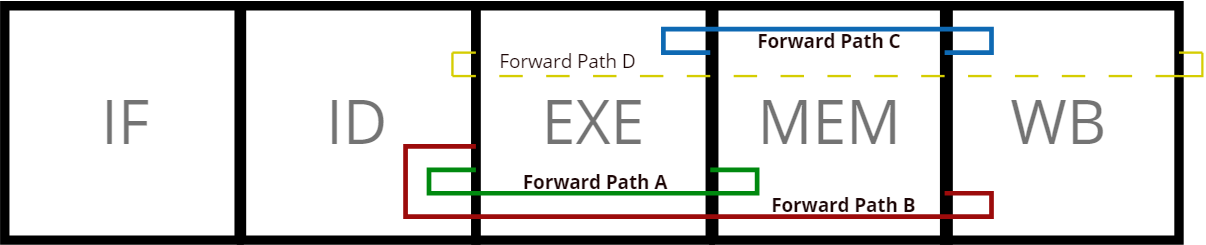
\includegraphics[width=1\textwidth]{FORWARDS}
		\caption{Forwarding Paths}
		\label{Image3.4}
	\end{center}
\end{figure}
\vspace{2mm}

The module is responsible for handling Forwards A,B, and C, while forward D\footnote{We will analyze the Forward D later.} is being handled by some external logic. So there are three main RAW scenarios that require resolution.

\subsubsection{Scenario A} 
\label{3.2.5.1}

\begin{lstlisting}[caption={Forward Path A Example},captionpos=b]
	OP_A	Reg_X, Reg_A, Reg_B
	OP_B 	Reg_Y, Reg_X, Reg_C
\end{lstlisting}



This scenario concerns the $ID$ and $Execute$ stages. OP\_A writes its result to Reg\_X. Then OP\_B requires Reg\_X's value as $rs1$ operand. Without the forwarding path, we would have to stall for at least two clock cycles and wait for OP\_A to reach the $Write\ Back$ stage. We know that the value that will be written at at Reg\_X will be available at the end of $Execute$ stage. So instead of stalling for two clock cycles, we activate the Forward Path A and transfer the value needed to OP\_B.

\clearpage

\subsubsection{Scenario B}
\label{3.2.5.2}

\begin{lstlisting}[caption={Forward Path B Example},captionpos=b]
	OP_A	Reg_X, Reg_A, Reg_B
	....	.....  .....  .....
	OP_B 	Reg_Y, Reg_X, Reg_C
\end{lstlisting}

This scenario concerns the $ID$ and $Memory$ stages. Once again OP\_A writes its result to Reg\_X and then, after one command that is in-between them, OP\_B requires this value as an operand. If not for the Forward Path B, we would have to stall again for one clock cycle and wait for OP\_A to reach the $Write\ Back$ stage.

\subsubsection{Scenario C}

\begin{lstlisting}[caption={Forward Path C Example},captionpos=b]
	LOAD 	Reg_X, IMM(Reg_A)
	STORE	Reg_X, IMM(Reg_B)
\end{lstlisting}

This scenario concerns only the $Memory$ stage. It only occurs when there is a $STORE$ command after a $LOAD$ command, of whom the later wishes to write in the memory the register value that the first has loaded. We would normally have to stall for one clock cycle again but with the Forward Path C we can overcome this issue. 

\subsubsection{Stall Generation}
\begin{lstlisting}[caption={Stall Scenario},captionpos=b]
LOAD 	Reg_X, IMM(Reg_A)
OP_A	Reg_A, Reg_X, Reg_B
\end{lstlisting}

In this case, we have to stall the OP\_A and those who follow, because the $LOAD$ command, has to reach the $Memory$ stage and then, activate the Forward Path B so that it can provide the needed value. This happens due to the nature of the $LOAD$ commands, which have their result ready at the end of $Memory$ stage and not at the $Execute$ stage like the other computational commands.\\

Here, we present an algorithm that represents the Stall \& Forward Predictor module's behavior. 

\begin{algorithm}[H]
	\SetAlgoLined
	\SetKwInOut{Input}{input}\SetKwInOut{Output}{output}
	
	\Input{ $RS1[4..0]$,$RS2[4..0]$, $RD\_IN\_EXE[4..0]$, $RD\_IN\_MEMORY[4..0]$, $LOAD\_IN\_EXE$, $CONTROL_WORD[20..18]$}
	\Output{ $FWDA$, $FWDB$, $FWDC$, $STALL$} 
	\BlankLine
	\BlankLine
	
	\emph{{\small $COMMAND\_IN\_ID \leftarrow f({\scriptsize CONTROL\_WORD[20..18]})$} {\footnotesize= (R/S/U/B/J)}} \;
	\BlankLine
	\If{$RS1$ == $RD\_IN\_EXE$ AND \underline{$RS1\neq REG_{0}$}} { \small $FWD\_A\_RS1 \leftarrow 1$\;}
	
	\If{$RS2$ == $RD\_IN\_EXE$ AND \underline{$RS2\neq REG_{0}$}} { \small $FWD\_A\_RS2 \leftarrow 1$\;}
	
	
	\If{IMM\_TYPE == "010"} { {\small $IMMEDIATE$ =  \underline{B-type} Immediate, f(\footnotesize{$FETCHED\_WORD$})} \;}
	\uElseIf{IMM\_TYPE == "011"} { {\small $IMMEDIATE$ =  \underline{U-type} Immediate, f(\footnotesize{$FETCHED\_WORD$})} \;}
	\uElseIf{IMM\_TYPE == "100"} { {\small $IMMEDIATE$ =  \underline{J-type} Immediate, f(\footnotesize{$FETCHED\_WORD$})} \;}
	\Else{ {\small $IMMEDIATE$ =  \underline{XXX..X}} \;}
	
	\caption{Stall and Forward Predictor Algorithm}
\end{algorithm}	
